
\documentclass[10pt]{article}
\usepackage[utf8]{inputenc}
\usepackage{kotex}
\usepackage{graphicx}
\usepackage{subfigure}
\usepackage{titling}
\setlength{\droptitle}{-2cm}
\usepackage{array}
\usepackage{amssymb}
\usepackage{amsmath}
\usepackage{siunitx} 
\usepackage{enumerate} 
\usepackage{pgfplots}
\usepackage{pgfplotstable}
\usepackage{tikz,pgfplots}
\usepackage{wasysym}
\usepackage{geometry}
\usepackage{authblk}
\usepackage{kotex}
\usepackage{bibunits}
\usepackage{tabularx}
\usepackage{hyperref}
\usepackage{pythonhighlight}

\geometry{
    a4paper,
    total={170mm,257mm},
    left=20mm,
    top=20mm,
}

\title{\textbf{Mathematical Foundation of DNN : HW 6}}
\author{Jeong Min Lee}

\begin{document}
\maketitle

\section*{1}
Let $D_p(\cdot)$ define as follows:

\begin{equation}
    D_p(x) = \begin{cases}
        0 \text{ with probability }p \\
        x/(1-p) \text{ with probability } 1-p
    \end{cases}
\end{equation}

For the case of ReLU and LeakyReLU, the dropout can be commutative. Let $f$ denote the ReLU Leaky ReLU.
\begin{align*}
    D_p(f(h)) &= \begin{cases}
        0 \text{ with probability } p \\
        f(h)/(1-p) \text{ with probability } 1-p
    \end{cases} \; (\because \text{the defition of dropout})\\&= \begin{cases}
        0 \text{ with probability } p \\
        f(h/(1-p)) \text{ with probability } 1-p
    \end{cases} \; (\because f(ax) = af(x)\; \forall x, a>0) \\ &= f(D_p(h))
\end{align*}
However, for the sigmoid, we cannot do same thing to the discussion above since it is not homogeneous function. 
In addition, there is a trivial counter-example. Consider the hidden layer with element $[0,0,1]$. If we do dropout first, 
the last node can be zero with probability $p$ and it results in $[0,0,0]$. Then, after applying the sigmoid function, the all three elements in the output must be same. 
However, if we do sigmoid activation first, since $Sigmoid(0) \neq 0 $, the intermediate layer would be $[\sigma(0),\sigma(0),\sigma(1)]$. 
Although dropout cannot change their value to be evenly, they are not same to the result of Dropout-Sigmoid.

\section*{2}
In this problem, I denote the bold symbol of each variable as the random variable corresponding to it. 
\begin{equation*}
    \mathbb{E}[\mathbf{x}^{(i)}] = 0,\quad \mathbb{E}\left[\left(\mathbf{x}^{(i)}\right)^2\right] = 1
\end{equation*}
From the PyTorch offficial document, it is important to note the following relations.
\begin{align*}
    \mathbf{A_l^{(ij)}} &\sim \mathcal{U}\left(-\sqrt{\frac{1}{n_{l-1}}},\sqrt{\frac{1}{n_{l-1}}}\right)\\
    \mathbf{b_l^{(i)}} &\sim \mathcal{U}\left(-\sqrt{\frac{1}{n_{l-1}}},\sqrt{\frac{1}{n_{l-1}}}\right)
\end{align*}
The relations above imply the following. 
\begin{align*}
    \mathbb{E}[\mathbf{A_l^{(ij)}}] &= 0, \quad \mathbb{E}[\mathbf{b_l^{(i)}}] = 0\\ 
    \mathbb{E}\left[\left(\mathbf{A_l^{(ij)}}\right)^2\right] &= \frac{1}{3n_{l-1}}, \quad \mathbb{E}\left[\left(\mathbf{b_l^{(i)}}\right)^2\right] = \frac{1}{3n_{l-1}} 
\end{align*}
Then, to derive the mean of $\mathbf{y}_L$, consider the mathematical induction of $\mathbb{E}[\mathbf{y}_l^{(i)}]$.
For the base case, the mean value of $\mathbf{y}^{(i)}_1$ is zero. 
\begin{align*}
    \mathbb{E}[\mathbf{y_1^{(i)}}] &= \mathbb{E}[\mathbb{E}[\mathbf{y}_1^{(i)}|x]] \\ &= \mathbb{E}\left[\sum_{j=1}^{n_0}\mathbb{E}\left[\mathbf{A}_l^{(ij)}\mathbf{x}^{(j)}|x\right] + \mathbb{E}\left[\mathbf{b_1^{(i)}}|x\right]\right] \\
    &= \mathbb{E}\left[\sum_{j=1}^{n_0} \mathbb{E}\left[\mathbf{A}_l^{(ij)}\right]x^{(j)}\right] \\
    &= 0
\end{align*}
Then, for the inductive step, the mean value of $\mathbf{y}^{(i)}_l$ is zero. To proof it, consider the following induction hypothesis: $\mathbb{E}[\mathbf{y}^{(i)}_{l-1}] = 0$.
\begin{align*}
    \mathbb{E}[\mathbf{y}_l^{(i)}] &= \mathbb{E}[\mathbb{E}[\mathbf{y}_l^{(i)}|y_{l-1}]]\\&= \mathbb{E}\left[\sum_{j=1}^{n_{l-1}} \mathbb{E}\left[\mathbf{A}_l^{(ij)}\mathbf{y}_{l-1}^{(j)}|y_{l-1}\right] + \mathbb{E}\left[\mathbf{b}_l^{(i)}|y_{l-1}\right]\right] \\
    &= \mathbb{E}\left[\sum_{j=1}^{n_{l-1}} \mathbb{E}\left[\mathbf{A}_l^{(ij)}\right]y_{l-1}^{(j)}\right] \\
    &= 0
\end{align*}
Next, I'll derive the variance of $\mathbf{y}^{(i)}_l$.
\begin{align*}
    \mathbb{E}\left[\left(\mathbf{y}_l^{(i)}\right)^2\right] &= \mathbb{E}\left[\mathbb{E}\left[\left(\mathbf{y}_l^{(i)}\right)^2|y_{l-1}\right]\right] \\ &= \mathbb{E}\left[\mathbb{E}\left[\left(\sum_{j}\mathbf{A}_l^{(ij)}\mathbf{y}_{l-1}^{(j)} + \mathbf{b}_l^{(i)}\right)^2\bigg|y_{l-1}\right]\right]\\
    &= \mathbb{E}\left[\mathbb{E}\left[\sum_j\sum_k \mathbf{A}_l^{(ij)}\mathbf{A}_l^{(ik)}\mathbf{y}_{l-1}^{(j)}\mathbf{y}_{l-1}^{(k)} + 2\mathbf{b}_l^{(i)}\sum_j \mathbf{A}_l^{(ij)}\mathbf{y}_{l-1}^{(j)} + \left(\mathbf{b}_l^{(i)}\right)^2\bigg|y_{l-1}\right]\right] \\
    &= \mathbb{E}\left[\mathbb{E}\left[\sum_j\sum_k \mathbf{A}_l^{(ij)}\mathbf{A}_l^{(ik)}\mathbf{y}_{l-1}^{(j)}\mathbf{y}_{l-1}^{(k)}\bigg|y_{l-1}\right] + \mathbb{E}\left[2\mathbf{b}_l^{(i)}\sum_j \mathbf{A}_l^{(ij)}\mathbf{y}_{l-1}^{(j)}\bigg|y_{l-1}\right] + \mathbb{E}\left[\left(\mathbf{b}_l^{(i)}\right)^2\bigg|y_{l-1}\right]\right]\\
    &= \mathbb{E}\left[\sum_j\sum_k \mathbb{E}\left[\mathbf{A}_l^{(ij)}\mathbf{A}_l^{(ik)}\bigg|y_{l-1}\right]y_{l-1}^{(j)}y_{l-1}^{(k)}\right] + \frac{1}{3n_{l-1}}\\
    &= \mathbb{E}\left[\sum_j\sum_k \frac{1}{3n_{l-1}}\delta_{jk}y_{l-1}^{(j)}y_{l-1}^{(k)}\right] + \frac{1}{3n_{l-1}} \\
    &= \sum_j \frac{1}{3n_{l-1}}\mathbb{E}\left[\left(\mathbf{y}_{l-1}^{(j)}\right)^2\right] + \frac{1}{3n_{l-1}}
\end{align*}
As the result above says, $\mathbb{E}\left[\left(\mathbf{y}_l^{(i)}\right)^2\right]$ actually doesn't depend on the index $i$. This implies that $\mathbb{E}\left[\left(\mathbf{y}_l^{(1)}\right)^2\right] = \mathbb{E}\left[\left(\mathbf{y}_l^{(2)}\right)^2\right] = \cdots = \mathbb{E}\left[\left(\mathbf{y}_l^{(n_l)}\right)^2\right]$.
From induction, this must be held on the $l-1$ layers.(Note that we can see the base case if we put $l=1$ on the last equation above). Thus, 
\begin{align*}
    \mathbb{E}\left[\left(\mathbf{y}_l^{(i)}\right)^2\right] &= \frac{1}{3}\mathbb{E}\left[\left(\mathbf{y}_{l-1}^{(i)}\right)^2\right] + \frac{1}{3n_{l-1}} \\
    \mathbb{E}\left[\left(\mathbf{y}_l^{(i)}\right)^2\right] &= \frac{1}{3}\left(\frac{1}{3}\left(\mathbb{E}\left[\left(\mathbf{y}_{l-2}^{(i)}\right)^2\right] + \frac{1}{n_{l-2}}\right) + \frac{1}{n_{l-1}}\right) \\ &\vdots \\ &= \frac{1}{3^l}\mathbb{E}\left[\left(\mathbf{y}_0^{(i)}\right)^2\right] + \sum_{k=0}^{l-1}\frac{1}{3^{l-k}n_k}\\
    \therefore \mathbb{E}\left[\left(\mathbf{y}_L^{(i)}\right)^2\right] &= \frac{1}{3^L} + \sum_{k=0}^{L-1}\frac{1}{3^{L-k}n_k}
\end{align*}
\section*{3}
I refer to the result of HW4-6 to solve this problem. 
\subsection*{i}
From the problem 6-(a) in HW4, we saw that ${\partial\over \partial y_{l-1}} \sigma(A_ly_{l-1}) + b_l = \text{diag}(\sigma^\prime(A_ly_{l-1} + b_l))A_l$. Thus,
\begin{align*}
    y_l &= \sigma(A_ly_{l-1} + b_l) + y_{l-1} \\
    {\partial y_l \over \partial y_{l-1}} &= \text{diag}\left(\sigma^\prime(A_ly_{l-1} + b_l)\right)A_l + I_m
\end{align*}
Here, $I_m$ denotes the identity with dimension $m$.
\subsection*{ii}
Since $b_l$ and $A_l$ are independent to $y_{l-1}$, we can directly use the result of problem 6 at HW4(with simple chain rule).
\begin{align*}
    {\partial y_L\over \partial b_l} &= {\partial y_L \over \partial y_l} {\partial y_l \over \partial b_l} = {\partial y_L \over \partial y_l} \text{diag}(\sigma^\prime(A_ly_{l-1} + b_l))\\
    {\partial y_L \over \partial A_l} &= \text{diag}(\sigma^\prime(A_ly_{l-1})+ b_l)\left({\partial y_L \over \partial y_l}\right)^T y_{l-1}^T
\end{align*}

\subsection*{iii}
Both ${\partial y_L\over \partial b_i}$ and ${\partial y_L \over \partial A_i}$ contain ${\partial y_L \over \partial y_i}$ term. According to the chain rule, 
\begin{align*}
    {\partial y_L\over \partial y_i} = {\partial y_L \over \partial y_{L-1}} \cdot {\partial y_{L-1} \over \partial y_{L-2}}\cdots {\partial y_{i+1} \over \partial y_{i}} = \prod_{k = i+1}^L {\partial y_k \over \partial y_{k-1}} = \prod_{k = i+1}^L \text{diag}\left( \sigma^\prime(A_ky_{k-1} + b_k) \right)A_k + I_m
\end{align*}
As the equations above tell, eventhough $A_j = 0 $ for some $j\in \left\{l+1, \cdots, L-1\right\}$ or $\sigma^\prime(A_jy_{j-1} + b_j) = 0$ for some $j \in \left\{l+1,\cdots, L-1\right\}$, the identity matrices are still alive. Thus, the derivatives do not have to be zero.
Note that the other components in both derivatives also are nonzero, in general.

\section*{4}
\subsection*{a}
In this problem, I used the following formula.
\begin{equation*}
    \text{trainable parameter} = (\text{kernel size})^2 \times C_{out} \times C_{in} + C_{out}
\end{equation*}
The overall calculation of the first convolution layer is as follow.
\begin{align*}
    &(128\times 1^2 \times 256 + 128) + (128 \times 3^2 \times 128 + 128) + (256\times 1^2 \times 128 + 256) = 213,504 \\
\end{align*}

For the second implementation, considering that each path have the same number of the trainable paramters, I calculated the number of trainable paramters for a single path. 
The whole calculation process is as follow.
\begin{align*}
    &(256\times 1^2 \times 4 + 4) + (4 \times 3^2 \times 4 + 4) + (4\times 1^2 \times 256 + 256) = 2456 \\
    &\therefore 32\times 2456 = 78,592
\end{align*}
\subsection*{b}
\begin{python}
class STMConvLayer(nn.Module):
    def __init__(self):
        super(STMConvLayer, self).__init__()
        self.layer1 = nn.ModuleList([
            nn.Conv2d(256,4,kernel_size =1, stride = 1)
            for i in range(32)
        ])
        self.layer2 = nn.ModuleList([
            nn.Conv2d(4,4,kernel_size = 3,stride = 1, padding = 1)
            for i in range(32)
        ])
        self.layer3 = nn.ModuleList([
            nn.Conv2d(4,256, kernel_size = 1, stride = 1)
            for i in range(32)
        ])
    def forward(self,x):
        out = []
        for i in range(32):
            x = torch.nn.functional.relu(self.layer1[i](x))
            x = torch.nn.functional.relu(self.layer2[i](x))
            x = torch.nn.functional.relu(self.layer3[i](x))
            out = out.append(x)
        return sum(out)
\end{python}
The structure of my STMConvLayer is as follow. The followings are produced by print() function.
\begin{python}
STMConvLayer(
  (layer1): ModuleList(
    (0-31): 32 x Conv2d(256, 4, kernel_size=(1, 1), stride=(1, 1))
  )
  (layer2): ModuleList(
    (0-31): 32 x Conv2d(4, 4, kernel_size=(3, 3), stride=(1, 1), padding=(1, 1))
  )
  (layer3): ModuleList(
    (0-31): 32 x Conv2d(4, 256, kernel_size=(1, 1), stride=(1, 1))
  )
)
\end{python}
\subsection*{5}
\begin{figure}[!h]
    \begin{center}
        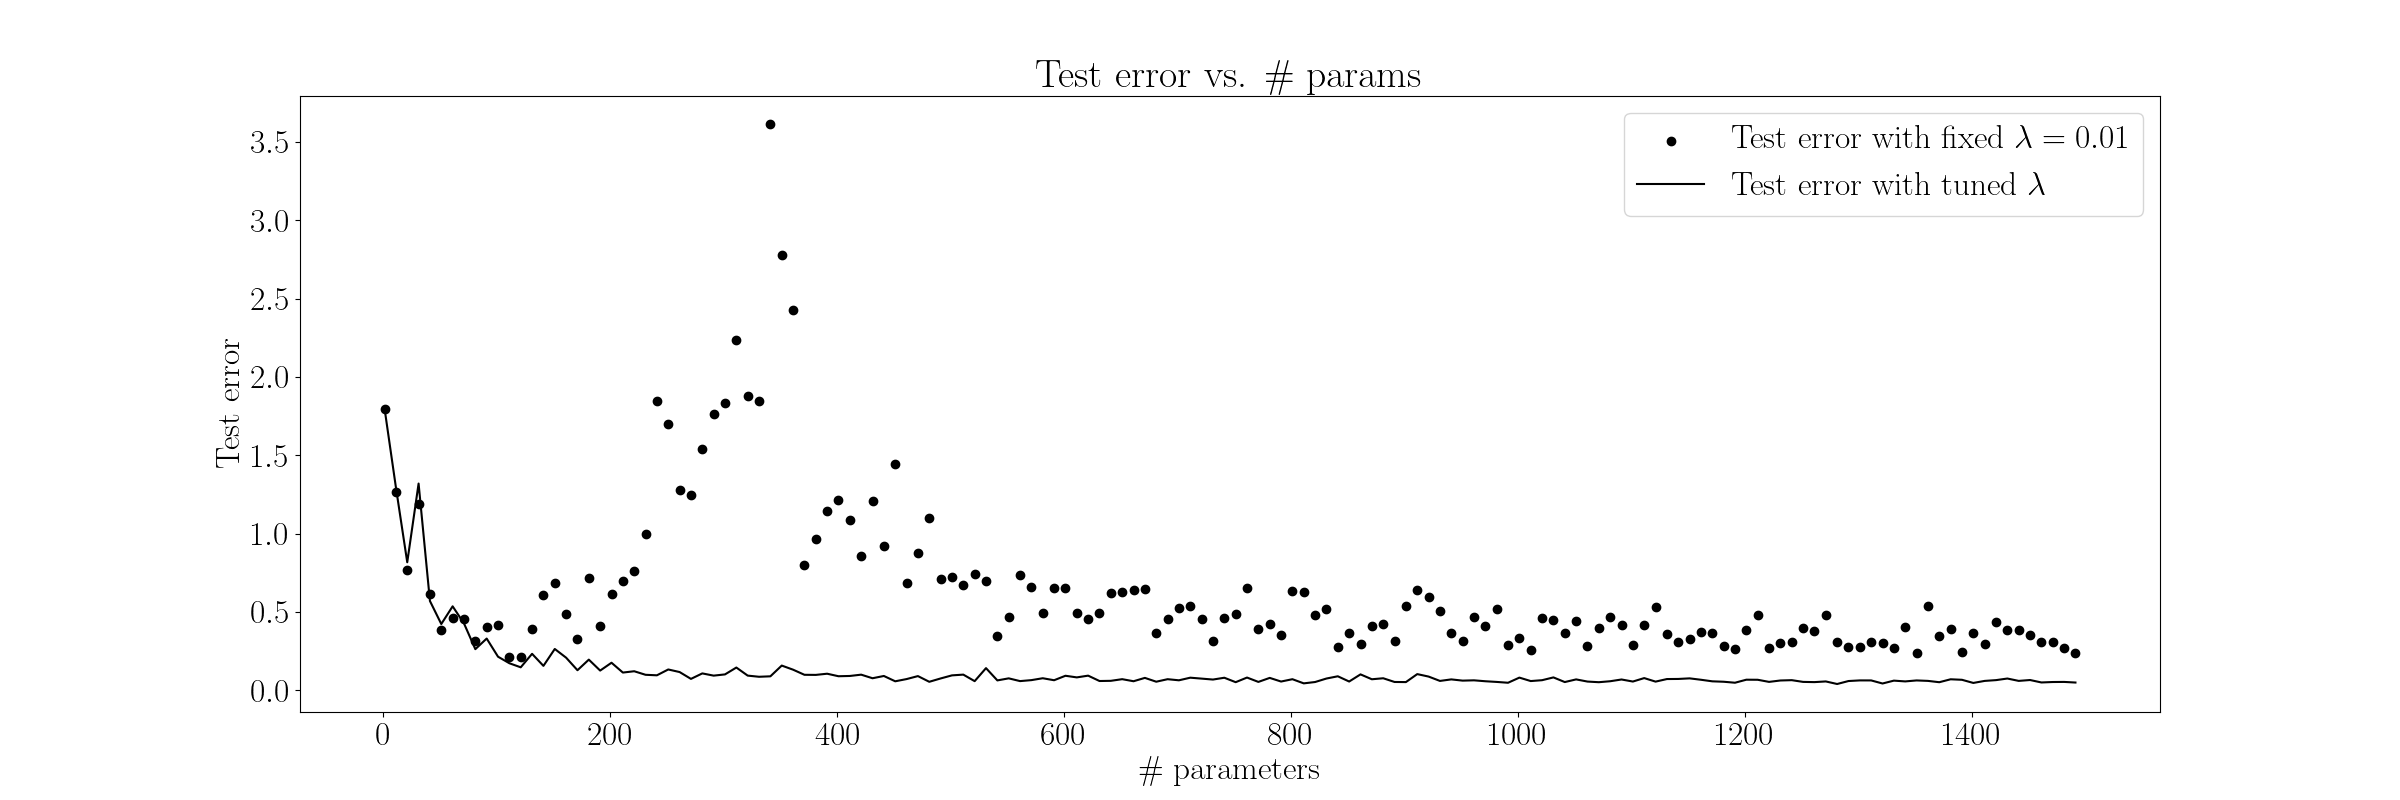
\includegraphics[scale = 0.25]{double_descent.png}
    \end{center}
\end{figure}


\begin{python}
import matplotlib.pyplot as plt 
import numpy as np 


"""
Step 1 : Generate Toy data
"""

d = 35
n_train, n_val, n_test = 300, 60, 30
np.random.seed(0)
beta = np.random.randn(d)
beta_true = beta / np.linalg.norm(beta)
# Generate and fix training data
X_train = np.array([np.random.multivariate_normal(np.zeros(d), np.identity(d)) for _ in range(n_train)])
Y_train = X_train @ beta_true + np.random.normal(loc = 0.0, scale = 0.5, size = n_train)
# Generate and fix validation data (for tuning lambda). 
X_val = np.array([np.random.multivariate_normal(np.zeros(d), np.identity(d)) for _ in range(n_val)])
Y_val = X_val @ beta_true 
# Generate and fix test data
X_test = np.array([np.random.multivariate_normal(np.zeros(d), np.identity(d)) for _ in range(n_test)])
Y_test = X_test @ beta_true 


"""
Step 2 : Solve the problem
"""    

lambda_list = [2 ** i for i in range(-6, 6)]
num_params = np.arange(1,1501,10)

errors_opt_lambda = []
errors_fixed_lambda = []
for p in num_params : 
    W = np.random.randn(p, d) / np.sqrt(p)

    # ReLU function
    X_train_transformed = np.maximum(X_train @ W.T, 0)
    X_val_transformed = np.maximum(X_val @ W.T, 0)
    X_test_transformed = np.maximum(X_test @ W.T, 0)

    # (X^TX + lambda I_p)theta = X^TY : normal equation
    theta_fixed_lambda = np.linalg.solve(X_train_transformed.T @ X_train_transformed + 0.01 * np.eye(p), X_train_transformed.T @ Y_train)
    errors_fixed_lambda.append(np.mean((X_test_transformed @ theta_fixed_lambda - Y_test) ** 2))

    val_errors = []
    for lambda_ in lambda_list:
        theta_opt_lambda = np.linalg.solve(X_train_transformed.T @ X_train_transformed + lambda_ * np.eye(p), X_train_transformed.T @ Y_train)
        val_errors.append(np.mean((X_val_transformed @ theta_opt_lambda - Y_val) ** 2))
    optimal_lambda = lambda_list[np.argmin(val_errors)]
    theta_opt_lambda = np.linalg.solve(X_train_transformed.T @ X_train_transformed + optimal_lambda * np.eye(p), X_train_transformed.T @ Y_train)
    errors_opt_lambda.append(np.mean((X_test_transformed @ theta_opt_lambda - Y_test) ** 2))
"""
Step 3 : Plot the results
"""    

plt.figure(figsize = (24, 8))
plt.rc('text', usetex = True)
plt.rc('font', family = 'serif')
plt.rc('font', size = 24)


plt.scatter(num_params, errors_fixed_lambda, color = 'black',
            label = r"Test error with fixed $\lambda = 0.01$",
            ) 
plt.legend()

plt.plot(num_params, errors_opt_lambda, 'k', label = r"Test error with tuned $\lambda$")
plt.legend()
plt.xlabel(r'$\#$ parameters')
plt.ylabel('Test error')
plt.title(r'Test error vs. $\#$ params')

plt.savefig('double_descent.png')
plt.show()
\end{python}

\end{document}